\section{The CMS Detector}
\label{sec:CMSdetector}

The CMS detector is a general purpose detector installed 100~m underground at the LHC interaction point 5 (P5) near the village of Cessy in France.
It has been designed to exploit the different properties of the wide range of particles and phenomena produced in high-energy collisions in the LHC.
The design of the CMS detector is driven by the challenges of a physics experiment in the LHC environment. 
Many of the physics benchmark channels have a small cross section and the background from QCD jet production is overwhelmingly dominant.
In order to achieve high rejection power with an optimal efficiency for rare channels, the detector has to be able to reconstruct the primary interaction entirely and to reduce the influence of overlapping events. Therefore, one needs to collect all possible information on the particles passing through the detector. Since these have different properties, a mixture of sub-detectors is required for a complete event reconstruction. The reconstruction of lepton signatures is essential for the extraction of rare processes and an excellent muon and electron identification and momentum resolution is desired. A precise measurement of secondary vertices and impact parameters is necessary for an efficient identification of heavy flavor quarks and $\tau$-leptons. Moreover, a large hermetic geometric coverage is preferred, which allows for a precise estimate of the transverse momentum carried away by invisible particles through the sum of all visible particles.

The high peak luminosities of LHC lead to large pileup imposing further challenges to the design. As a consequence of pileup, the products of an interaction under study may be confused with those from other interactions in the same bunch crossing. This effect can be reduced by using high-granularity detectors resulting in low occupancy. In addition, the short bunch crossing requires fast response time and good time resolution of each detector element in order to discriminate the interaction under study from the interactions occurring in neighbouring bunch crossings. Hence, a large number of detector channels and an excellent synchronization among them are required. Another challenge arises from the large flux of particles near the interaction point which leads to high radiation levels and the need of radiation hard detectors and front-end electronics.\\

Figure~\ref{fig:CMSlayout} shows the layout of the CMS detector. The detector is built in a cylindrical structure composed of a barrel in the center and endcaps at both sides. This structure is 21.6-m-long, 14.6-m in circumference and 12500-tons-heavy. The detector design and layout was driven by the choice of the magnetic field configuration. Large bending power is needed for a precise measurement of the momentum of high-energy charged particles. Within the CMS detector this is achieved by a superconducting solenoid with a length of 12.9~m and an inner diameter of 5.9~m generating a magnetic field of 4~T. The bore of the magnet coil is large enough to accommodate the inner tracker and the calorimetry inside. 
The inner tracker consists of a pixel and a strip detector both made out of Silicon, and it is the key component of CMS to measure the momenta of charged particles and identify primary and secondary vertices. The calorimetry system comprises a crystal electromagnetic calorimeter (ECAL) and a brass and scintillator hadronic calorimeter (HCAL), which provide information on the energies and directions of all charged and neutral particles. Outside the magnet are the large muon detectors, which, integrated inside the return yokes of the magnet, provide identification of muons and measurement of their momenta.\\

For the description of the CMS detector the following coordinate system is used. The origin is centered at the nominal collision point inside the experiment with the $y$-axis pointing vertically upward, the $x$-axis pointing radially inward toward the center of the LHC, and the $z$-axis points along the beam direction. The azimuthal angle $\phi$ is measured from the $x$-axis in the $x$-$y$ plane. The polar angle $\theta$ is measured from the $z$-axis. Pseudorapidity is defined as $\eta$ = -ln~tan($\theta$/2). Thus, the momentum and energy measured transverse to the beam direction, denoted by \PT and \ET, respectively, are computed from the $x$ and $y$ components.\\

In the following sections the three main components of the CMS detector will be described together with a section on the triggering system.

\begin{figure}[h]
 \begin{center}
  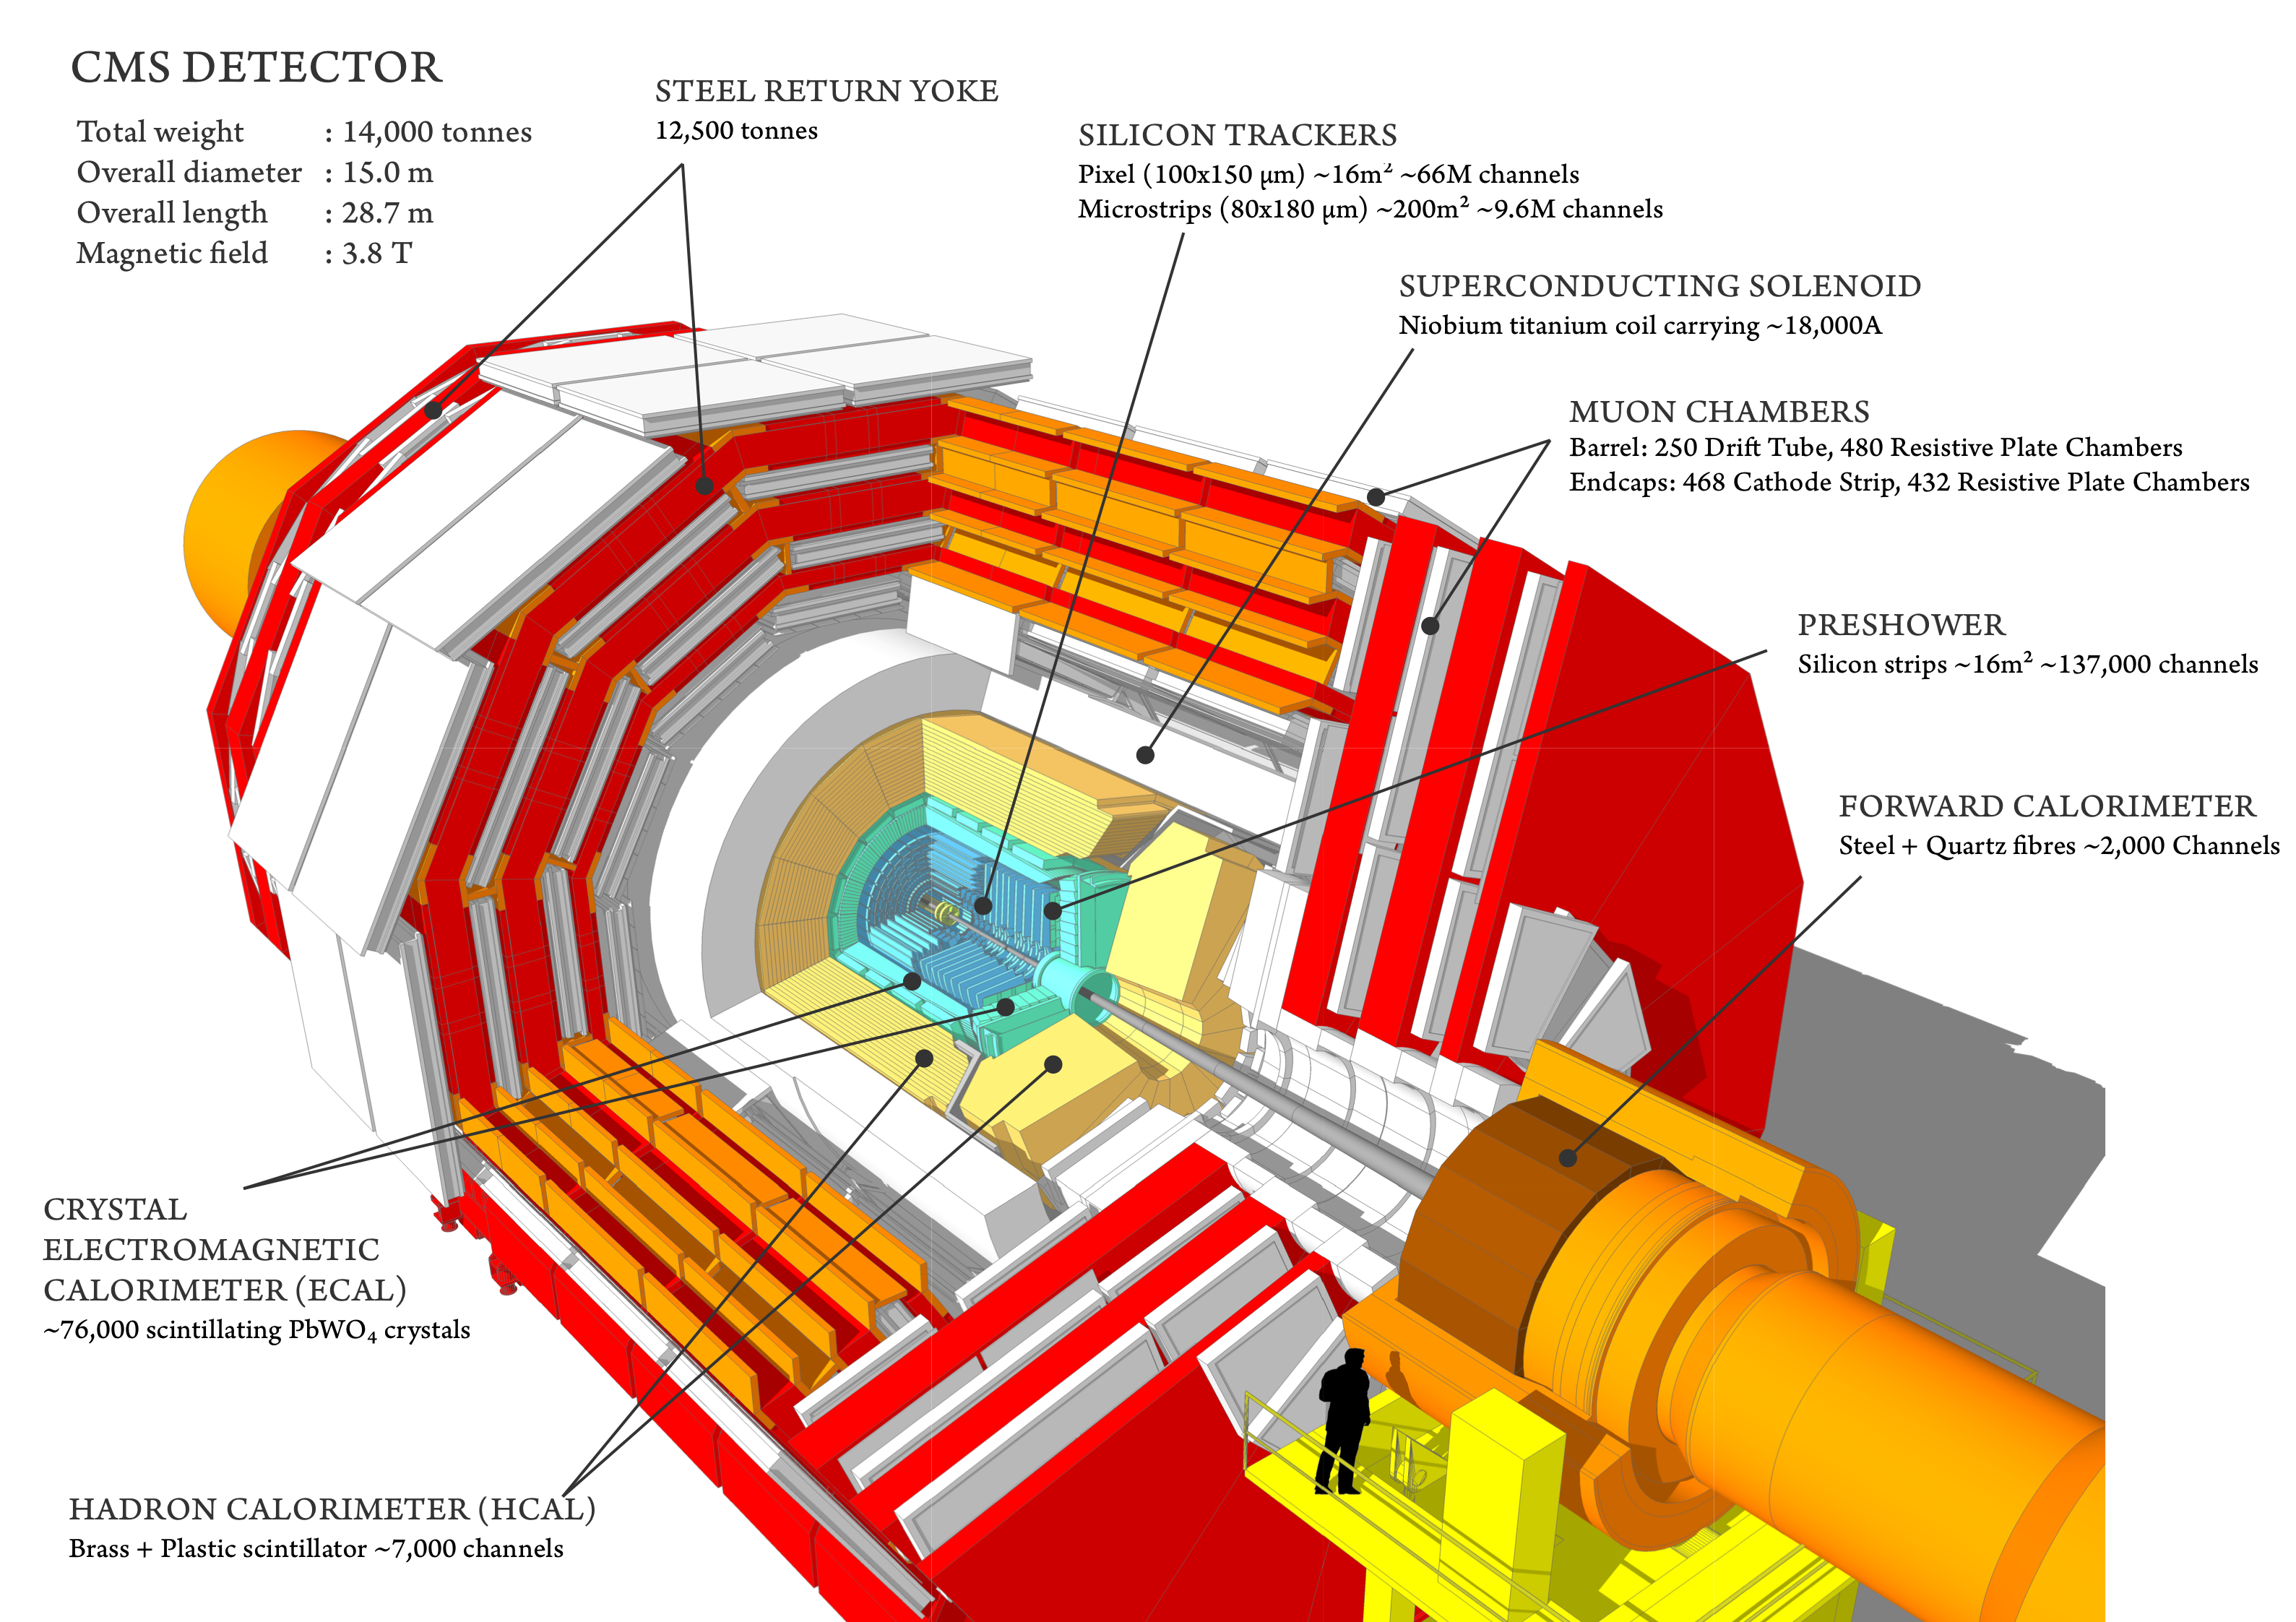
\includegraphics[width=0.9\textwidth]{\chthree/cms_120918_03.png}
 \end{center}
 \caption{\small Layout of the CMS experiment and its sub-detectors.}
 \label{fig:CMSlayout}
\end{figure}

\subsection{Tracking detectors}

The tracking system of CMS (Fig.~\ref{fig:TrackerLayout}) is designed to provide a precise and efficient measurement of the trajectories of charged particles emerging from the LHC collisions, as well as a precise reconstruction of secondary vertices~\cite{Karim�ki:368412}. It surrounds the interaction point and has a length of 5.8~m and a diameter of 2.5~m providing coverage up to $|\eta|~<$~2.5. In order to achieve high tracking efficiency at the high luminosities of LHC, a detector technology featuring granularity, speed and radiation hardness is required. Furthermore, the material budget of the tracking system has to be as low as possible in order to avoid a worsening of the tracking efficiency and resolution due to material interaction effects of the charged particle, such as multiple scattering, bremsstrahlung, photon conversion or nuclear interactions. These requirements lead to a tracker design entirely based on silicon detector technology. With about 200 m$^2$ of active silicon area the CMS tracker is the largest silicon tracker ever built. It is divided into a pixel detector close to the interaction region and a strip detector in the outer region.
At LHC design luminosity more than 1000 particles are hitting the tracking volume in each bunch crossing. This leads to a hit rate density of 1~MHz/mm$^2$ at a radius of 4~cm which imposes severe challenges to the design of the tracking detectors. With a pixel size of 100~$\times$~150~$\mu$m$^2$ in $r$-$\phi$ and $z$, respectively, an occupancy of the order of 10$^{-4}$ per pixel and LHC bunch crossing can be achieved. The hit rate density falls with the distance from the interaction point to 60~kHz/mm$^2$ at a radius of 22~cm and to 3~kHz/mm$^2$ at a radius of 115 cm. Therefore, at intermediate radii (20--55~cm), silicon micro-strip detectors are used, with a typical cell length of 10~cm and a pitch of 80~$\mu$m. At the outermost radii (55-110~cm)
the strip size can be further increased to 25~cm~$\times$~180~$\mu$m. With this choice an occupancy of less than 3\% is maintained in the strip detector.
However, the strip capacitance scales with its length and therefore the electronics noise is a linear function of the strip length as well, becoming not negligible in the outermost region where the strip size is the largest. In order to maintain a good signal to noise ratio of well above 10, CMS uses thicker silicon sensors for the outer tracker region (500~$\mu$m thickness as opposed to the 320~$\mu$m in the inner tracker) with correspondingly higher signal. To mitigate the radiation damage effects and prolong the lifetime of the detector modules, the tracking detectors are designed to run at subzero temperatures. The cooling is established using a mono-phase liquid cooling system with C$_6$F$_{14}$ as cooling fluid. The whole tracker system operated at +4$^\circ$C during Run 1. After this phase, several improvements have been implemented and an operative temperature of -15$^\circ$C is currently maintained for Run 2.\\

\begin{figure}[h]
 \begin{center}
  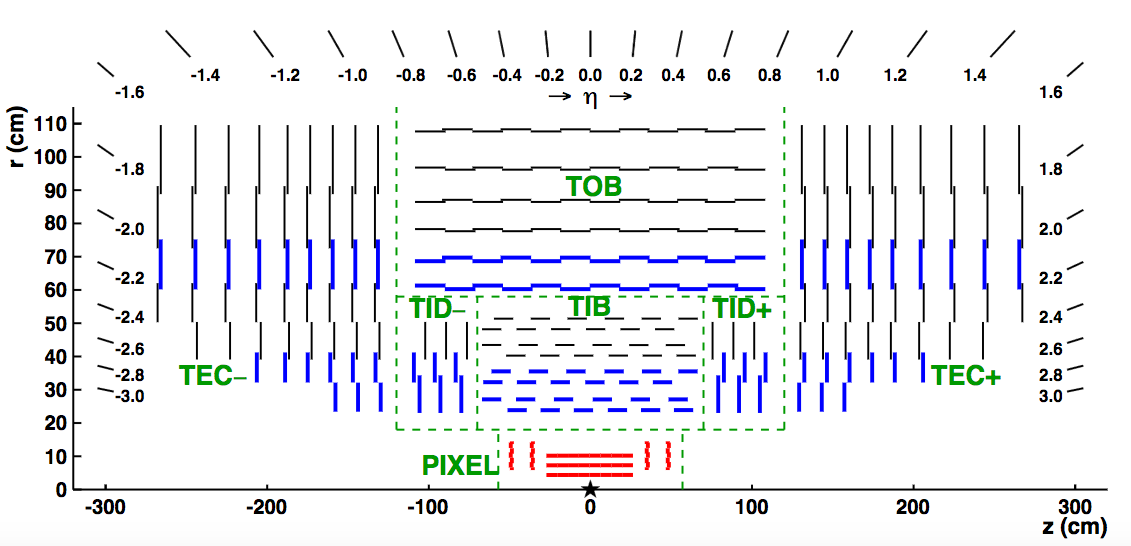
\includegraphics[width=0.8\textwidth]{\chthree/tracker.png}
 \end{center}
 \caption{\small Longitudinal section of half of the CMS Tracker system; the different detector types are indicated.}
 \label{fig:TrackerLayout}
\end{figure}

The pixel detector is built from 3 barrel layers at radii of 4.4, 7.3 and 10.2~cm (BPix) and two end disks (FPix) on each side at a distance of $z$ = $\pm$34.5, $\pm$46.5~cm from the interaction point. It consists of 1440 segmented silicon sensor modules with a total of 66 million readout channels covering an area of about 1~m$^2$. The pixel detector is essential for the reconstruction of secondary vertices from bottom quarks and $\tau$ leptons decays. It provides precise tracking points in $r$-$\phi$ and $z$ and therefore is responsible for a small impact parameter resolution that is important for good secondary vertex reconstruction. This is achieved thanks to the read out of the analog pulse height information. The sensor surface in the barrel layers is parallel to the magnetic fields, hence the charge carriers produced by a particle traversing experience a Lorentz drift, which leads to charge spreading over more than one pixel. The analog pulse height information can be used to calculate a center of gravity of the charge distribution improving the hit information. The forward detectors are tilted at 20$^\circ$ in a turbine-like geometry to induce charge-sharing. As shown in Fig.~\ref{fig:pxRes}, a spatial resolution of 10~$\mu$m in the transverse plane and 30~$\mu$m in the longitudinal plane can be achieved for BPix. For FPix a spatial resolution of 20~$\mu$m is obtained. %FROM TDR: A spatial resolution of approximately 15~$\mu$m in both the $r$-$\phi$ and $z$ directions can be achieved with charge-sharing between neighboring pixels. 
A detailed description of the design and the functioning of the CMS pixel barrel detector is given in Chapter~\ref{ch:BPixIntro}.\\

\begin{figure}[h]
 \begin{center}
   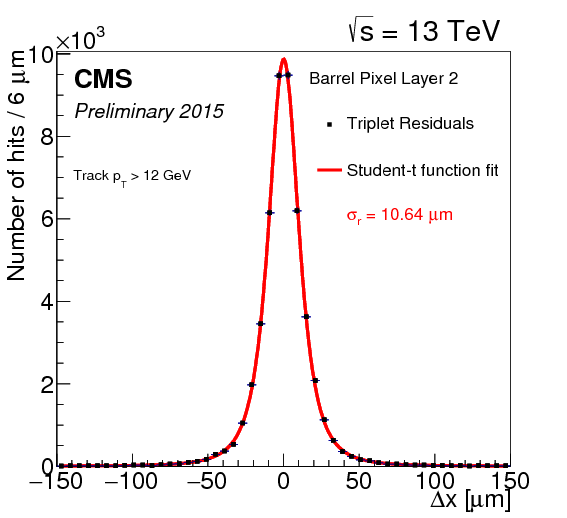
\includegraphics[width=0.48\textwidth]{\chthree/PixelResolution_dx.png}
  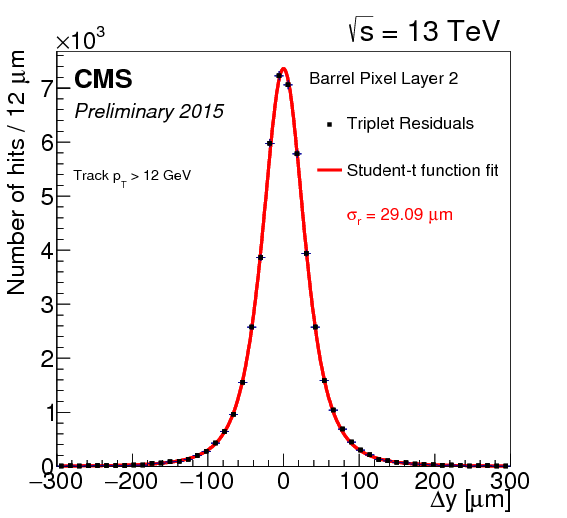
\includegraphics[width=0.48\textwidth]{\chthree/PixelResolution_dy.png}
 \end{center}
 \caption{Distribution of hit residuals on pixel barrel layer 2 in the transverse (left) and longitudinal (right) direction with respect to the beam. The distributions are fitted with a Student's t-function for which sigma is shown on the plot~\cite{PixelOffline2015}.}
 \label{fig:pxRes}
\end{figure}

The strip detector occupies the radial region between 20~cm and 1.16~m. As illustrated in Fig.~\ref{fig:TrackerLayout}, it is composed of four subsystems: the four-layer Tracker Inner Barrel (TIB), the six-layer tracker outer barrel (TOB) and on each side three-disk Tracker Inner Disks (TID) and nine-disk Tracker Endcaps (TEC). The silicon micro-strip sensors have strips parallel to the beam axis in the barrel and radial on the disks. The modules in the first two layers and rings, respectively, of TIB, TID, and TOB as well as rings 1, 2, and 5 of the TECs carry a second micro-strip detector module which is mounted back-to-back with a stereo angle of 100 mrad in order to provide a measurement of the second co-ordinate ( $z$ in the barrel and $r$ on the disks). This tracker layout ensures at least 9 hits in the silicon strip tracker in the full range of $|\eta|<$~2.4 with at least 4 of them being two-dimensional measurements.
The total number of silicon sensors in the strip tracker is 24244, making up a total active area of 198 m$^2$, with about 9.3 million of strips.\\
%TIB/TID
%The Tracker Inner Barrel and Disks (TIB/TID) extend in radius towards 55 cm and are composed of 4 barrel layers, supplemented by 3 disks at each end. TIB/TID delivers up to 4 $r$-$\phi$ measurements on a trajectory using 320 $\mu$m thick silicon micro-strip sensors with their strips parallel to the beam axis in the barrel and radial on the disks.  The strip pitch is 80 $\mu$m on layers 1 and 2 and 120 $\mu$m on layers 3 and 4 in the TIB, leading to a single point resolution of 23 $\mu$m and 35 $\mu$m, respectively.
%In the TID the mean pitch varies between 100 $\mu$m and 141 $\mu$m.
%TOB
%The TIB/TID is surrounded by the Tracker Outer Barrel (TOB). It has an outer radius of 116 cm and consists of 6 barrel layers of 500 $\mu$m thick micro-strip sensors with strip pitches of 183
%$\mu$m on the first 4 layers and 122 $\mu$m on layers 5 and 6. It provides another 6 $r$-$\phi$ measurements with single point resolution of 53 $\mu$m and 35 $\mu$m, respectively. 
%The TOB extends in $z$ between $\pm$ 118 cm. 
%TEC
%Beyond this $z$ range the Tracker EndCaps (TEC+ and TEC- where the sign indicates the location along the $z$ axis) cover the region 124 cm < |$z$| < 282 cm and 22.5 cm < |$r$| < 113.5 cm. Each TEC is composed of 9 disks, carrying up to 7 rings of silicon micro-strip detectors (320 $\mu$m thick on the inner 4 rings,  500 $\mu$m thick on rings 5-7) with radial strips of 97 $\mu$m to 184 $\mu$m average pitch. Thus, they provide up to 9 $\phi$ measurements per trajectory.
%In addition, the modules in the first two layers and rings, respectively, of TIB, TID, and TOB as well as rings 1, 2, and 5 of the TECs carry a second micro-strip detector module which is
%mounted back-to-back with a stereo angle of 100 mrad in order to provide a measurement of the second co-ordinate ( $z$ in the barrel and $r$ on the disks). The achieved single point resolution of this measurement is 230 $\mu$m and 530 $\mu$m in TIB and TOB, respectively, and varies with pitch in TID and TEC. This tracker layout ensures at least 9 hits in the silicon strip tracker in the full range of |$\eta$| < 2.4 with at least 4 of them being two-dimensional measurements (figure 3.2).

\subsection{Calorimetry}

The calorimeter measures the energies and directions of all neutral and charged particles traversing the detector, with the exception of muons and neutrinos. It consists of two parts, the
electromagnetic calorimeter (ECAL)~\cite{ECALtdr} and the hadronic calorimeter (HCAL)~\cite{HCALtdr}.\\

The goal of ECAL is to measure precisely the energy of electrons and photons which generate electromagnetic showers inside it. It is a hermetic and homogeneous calorimeter with a large pseudorapidity coverage up to $|\eta|<$~3. As illustrated in Fig.~\ref{fig:ECALLayout}, ECAL is divided into barrel and endcap detectors consisting of scintillation crystals made from lead tungstate (PbWO4). The choice of this material is motivated by its high density (8.28~g/cm$^3$ ), short radiation length ($X_0$ = 0.89~cm) and small Moli\`{e}re radius (2.2~cm), resulting in a high stopping power, fine granularity and therefore a compact calorimeter able to fit inside the solenoid.
The ECAL comprises 61200 crystals in the barrel and 7324 crystals in each of the 2 endcaps, for a total volume of 8.14~m$^3$ and 2.9~m$^3$, respectively. The crystals have a tapered shape and are mounted in a quasi-projective geometry.
The barrel extends radially between 1.29 and 1.75~cm covering the region $|z|<$~3.05~m and $|\eta|<$~1.479. The crystals have a front face cross-section of 22$\times$22~mm$^2$ and a length of 2.3~cm (25.8 $X_0$). They are organisezd in 36 identical supermodules each covering 20$^\circ$ in $\phi$. The crystals are contained in a thin-walled glass-fibre alveola structures (``submodules'') with 2($\phi$)$\times$5($\eta$) crystals per each resulting in a granularity 360-fold in $\phi$ and 2$\times$85-fold in $\eta$. The endcaps are placed at a distance of 3.14~m from the interaction point and they extend radially between 3.16 and 17.11~cm, covering the region 1.479 $<|\eta|<$ 3.0. The crystals have a front face cross section of 28.6$\times$28.6~mm$^2$ and a length of 2.2~cm (24.7 $X_0$). A preshower detector with a thickness of 3 $X_0$ is placed in front of the endcaps (1.653 $<|\eta|<$ 2.6) to guarantee a reliable discrimination of single photons and photons produced in pairs in neutral pion decays.
The relatively low light yield of the crystals (30~$\gamma$/MeV) requires use of photodetectors with intrinsic gain that can operate in a magnetic field. Silicon avalanche photodiodes (APDs) are used as photodetectors in the barrel and vacuum phototriodes (VPTs) in the endcaps. The light output and the amplification have a strong temperature dependence. The response to an incident electron changes by (3.8$\pm$0.4)\%/$^\circ$C which in turn means that the temperature has to be closely monitored and kept stable to a precision of $\pm$0.05$^\circ$C. The nominal operating temperature of the ECAL is 18$^\circ$C and is provided by a water cooling system.

The energy resolution of the electromagnetic calorimeter can be parametrized by the following expression:

\begin{equation}
\frac{\sigma_E}{E} = \frac{S}{\sqrt{E(\GeV)}} \oplus \frac{N}{E(\GeV)} \oplus C.
\end{equation}

The first term is stochastic including contributions from the shower containment, the number of photoelectrons and
the fluctuations in the gain process. The second contribution corresponds to the noise term, which includes noise in the readout electronics and fluctuations in pile-up.
The third term is a constant and dominates the energy resolution for high-energy electron and photon showers, depends
on non-uniformity of the longitudinal light collection, energy leakage from the back of the calorimeter, single-channel response uniformity and stability. 
The value of the three coefficients were determined by a electron test beam measurement in a matrix of 3�3 crystals to be S = 2.8\%, N = 12\% and C = 0.3\%~\cite{1748-0221-2-04-P04004}.
%This result was obtained reconstructing the showers in a matrix of 3$\times$3 crystals where the electron impact point on the calorimeter was tightly localized in a region of 4 mm $\times$ 4 mm to give maximum containment of the shower energy within the 3$\times$3 crystal matrix.  

\begin{figure}[h]
 \begin{center}
  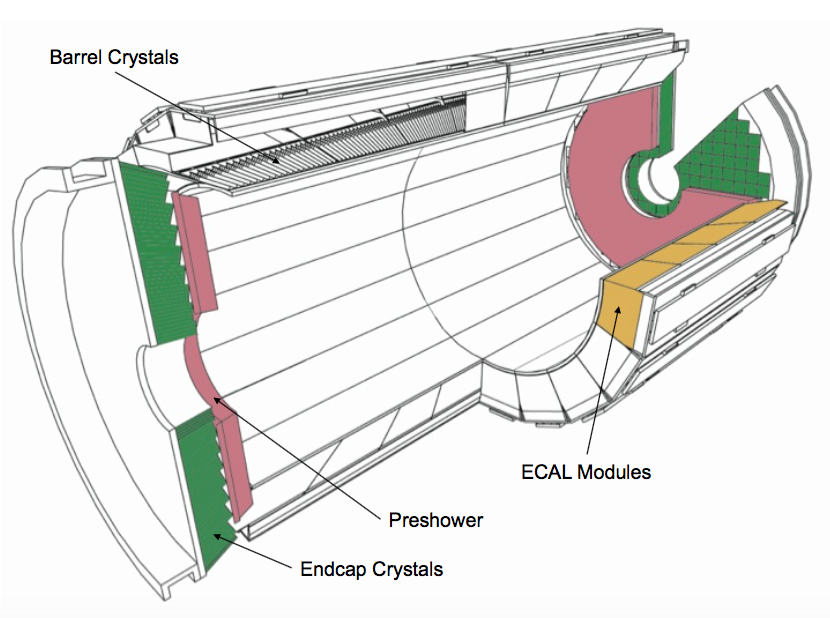
\includegraphics[width=0.8\textwidth]{\chthree/ECAL.png}
 \end{center}
 \caption{\small Schematic view of the CMS Electromagnetic Calorimeter~\cite{Chatrchyan:2008zzk}.}
 \label{fig:ECALLayout}
\end{figure}

The energy measurement of the ECAL is complemented by the measurement of the hadronic calorimeter.
%which aims at measuring the energy of the individual hadrons produced in each collision.
The HCAL is designed to be as near to hermetic around the interaction region as possible to allow events with missing energy to be identified.
It is a sampling calorimeter composed of layers of brass absorber interlaced with tiles of plastic scintillators as active material to detect the showers generated by the hadrons in the brass. The energy released in the scintillator tiles causes them to emit blue-violet light, a fraction of which is absorbed and re-emitted by embedded wavelength-shifting fibres in the green region of the spectrum. The green light is then carried by special fibre-optic waveguides to the readout system. The photodetection readout is based on multi-channel hybrid photodiodes (HPDs), photodetectors configured especially for CMS that can provide gain and operate in a high magnetic field. Figure~\ref{fig:HCALLayout} shows a schematic cross section of the HCAL detectors. The hadron barrel (HB) and endcaps (HE) calorimeters sit behind the tracker and the electromagnetic calorimeter as seen from the interaction point. The HB is radially restricted between the outer extent of the electromagnetic calorimeter ($r$ = 1.77~m) and the inner extent of the magnet coil ($r$ = 2.95~m). This constrains the total amount of material which can be put in to absorb the hadronic shower. Therefore, an Outer Hadron (HO) calorimeter is placed outside the solenoid complementing the barrel calorimeter. The HO uses the solenoid as additional absorbing material and provides sufficient containment for hadronic showers with a thickness of 11.8 interaction lengths ($\lambda_l$). The first scintillators are placed in front of the first absorber plate in order to sample showers developing in the material between the ECAL and the HCAL, while the last scintillators are installed after the last absorber plate to correct for late developing showers leaking out. 70000 and 20916 scintillator tiles are installed in the HB and the HE, respectively. The HB and HE cover the region $|\eta|<$~1.3 and 1.3~$<|\eta|<$~3.0, respectively.  Beyond $|\eta|$ = 3, the Hadron Forward (HF) calorimeter placed at 11.2~m from the interaction point extends the pseudorapidity coverage down to $|\eta|$ = 5.2.
The barrel depth goes from 5.46 $\lambda_l$ at $\eta$ = 0 to 10.8 at $\eta$ = 1.3, while the endcaps coincide with an average of 11 $\lambda_l$. The calorimeter is segmented and
arranged in towers as summarized in Table~\ref{tab:hcal}. The HF is positioned at a longitudinal distance of 11.2 m from the interaction point. It will experience unprecedented particle fluxes with an energy of 760 GeV deposited on average in a proton-proton interaction at ps = 14 TeV. This energy has to be compared to the average of 100 GeV deposited in the rest of the detector. The situation is even more severe as the energy is not spread equally among the HF, but has a pronounced peak at the highest rapidity. The HF is a sampling calorimeter made from steel absorber plates composed of 5mm thick grooved plates with quartz fibers inserted as active medium. The signal is generated when charged shower particles above the threshold generate Cherenkov light in the quartz fibres, thereby rendering the calorimeter mostly sensitive to the electromagnetic component of showers.

The HCAL energy resolution is 

\begin{equation}
\frac{\sigma_E}{E} = \frac{a}{\sqrt{E(GeV)}} \oplus 5\%
\end{equation}

where a is 65\% in the barrel, 85\% in the endcaps and 100\% in the forward calorimeter.

\begin{table}[htb]
\centering
\caption{Tower segmentation in azimuthal and polar angle for the hadronic barrel, endcap and forward calorimeter.}
\begin{tabular}{cccccc}
\hline
                                              & HB/HO                      & HE ($|\eta|\leq$2.5) & HE ($|\eta|>$2.5)     & HF ($|\eta|\leq$4.7) & HF ($|\eta|>$4.7) \\ \hline
$\Delta\phi\times\Delta\eta$  & 0.087$\times$0.087 & 0.087$\times$0.087 & 0.175$\times$0.175 & 0.175$\times$0.175 & 0.175$\times$0.35\\ \hline
\end{tabular}
\label{tab:hcal}
\end{table}

\begin{figure}[h]
 \begin{center}
  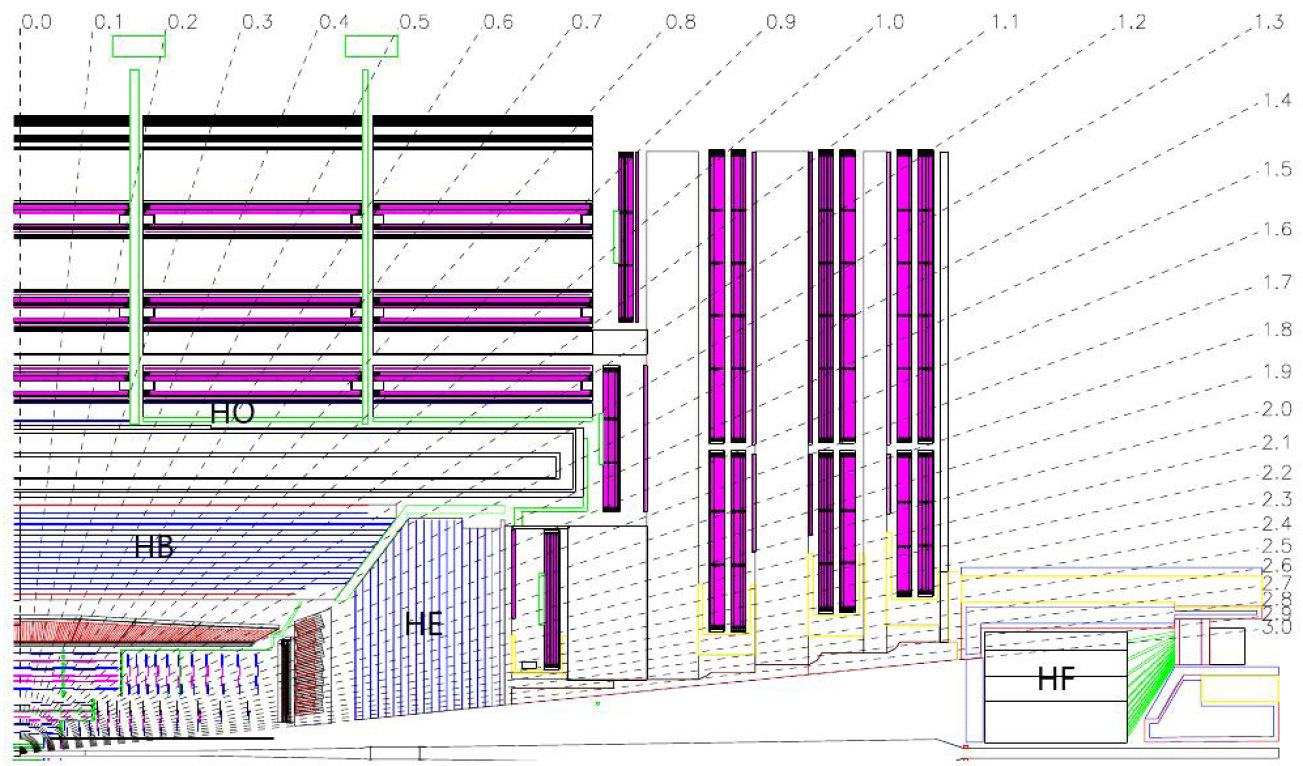
\includegraphics[width=0.8\textwidth]{\chthree/HCAL.png}
 \end{center}
 \caption{\small  Longitudinal view of the CMS detector showing the locations of the hadron barrel (HB), endcap (HE), outer (HO) and forward (HF) calorimeters~\cite{Chatrchyan:2008zzk}.}
 \label{fig:HCALLayout}
\end{figure}

\subsection{Muon detectors}\label{subsec:muonchambers}

The muon system is the outermost part of the CMS detector. It is located in the steel return yoke of the solenoid, covering the pseudorapidity region $|\eta|~<$~2.4. This is possible because muons are hardly affected by this large material budget. The coil acts as a shield from electromagnetic and hadronic particles escaping the calorimeters and the yoke provides a magnetic field between consecutive muon stations, allowing a momentum measurement independent from the inner tracker. The muon system is designed for three major functions: robust and fast identification of muons, good resolution of momentum measurement, and integration to a fast and reliable trigger system. The gaseous detectors has been chosen as muon detectors since they are robust and with a relative fast response. Furhermore, the area to be covered is extremely wide and a gaseous detector system allows to reduce the cost and the amount of readout channels. The muon system is thus composed of three types of gaseous detectors arranged in barrel and endcap sections, as shown in Fig.~\ref{fig:MuonSystem}: Drift Tubes (DTs), Resistive Plate Chambers (RPCs) and Cathode Strip Chambers (CSCs). The choice of different detector topologies lies essentially in the different expected particle rates. 

In the barrel region, where the neutron-induced background is small, the muon rate is low, and the 4-T magnetic field is uniform, DTs with standard rectangular drift cells are used covering the pseudorapidity region $|\eta|<$~1.2. A DT cell is a 4 cm wide gas tube with a positively charged stretched wire inside. 
The barrel DT chambers are organized in five separate wheels. Each wheel is divided into 12 sectors, each covering a 30$^\circ$ azimuthal angle. In each of the 12 sectors there are 4 chambers per wheel which are concentric around the beam line and separated by the iron return yoke. Each DT chamber, on average 2~m $\times$ 2.5~m in size, consists of 12 layers of DT cells, arranged in three groups of four. For the first 3 stations in each wheel, the middle group measures the $z$ coordinate while the two outside groups measure the $r$-$\phi$ coordinate. The fourth and outermost station does not contain the $z$-measuring planes. Each one of the 250 DT chambers has a resolution of $\sim$ 100~$\mu$m in $r$-$\phi$ and up to 150~$\mu$m in $z$, and can measure the particle direction with 1 mrad accuracy.

In the two endcap regions of CMS, where the muon rates and background levels are high and the magnetic field is large and non-uniform, CSCs are used with their fast response time, fine segmentation, and radiation resistance, covering the pseudorapity region between 0.9 and 2.4. 
Each CSC is trapezoidal shaped multiwire proportional chambers which consists of 6 gas gaps, each gap having a plane of radial cathode strips and a plane of anode wires running almost perpendicularly to the strips. The gas ionization and subsequent electron avalanche caused by a charged particle traversing each plane of a chamber produces a charge on the anode wire and an image charge on a group of cathode strips. Thus, each CSC provides a two-dimensional position measurement, where the $r$ and $\phi$ coordinates are determined by the cathode strips and the anode wires, respectively. 540 CSC are arranged in 4 disks per endcaps divided in concentric rings (3 rings in the innermost station, 2 in the others). Each chamber has a spatial resolution of about 200 mm in $r$, and 75$\times$150 $\mu$m in the $r$-$\phi$ coordinate.

In addition, there is a total of 610 RPCs added in both the barrel and endcap regions to provide a fast, independent, and highly-segmented trigger over a large portion of the rapidity range ($|\eta|<$~1.6) of the muon system. They produce a fast response, with good time resolution ($\sim$ 2 ns) but coarser position resolution than the DTs or CSCs. RPCs are made from two high resistive plastic plates with a voltage applied and separated by a gas volume. The signal generated by the muon when passing through the gas volume is detected by readout strips mounted on top of one of the plastic plates. Six layers of RPCs are installed in the barrel muon system, two layers in each of the first two stations and one layer in each of the last two stations. One layer of RPCs is built into each of the first three stations of the endcap.

\begin{figure}[h]
 \begin{center}
  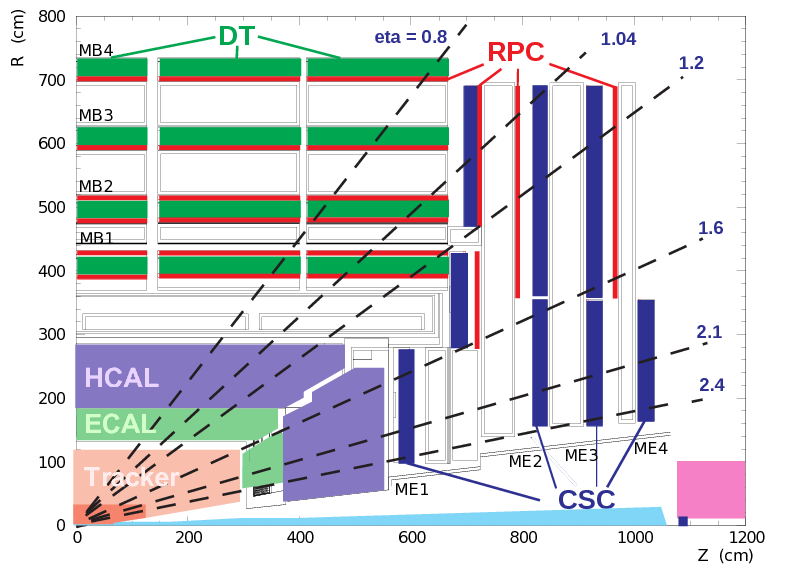
\includegraphics[width=0.8\textwidth]{\chthree/MuonSystem.png}
 \end{center}
 \caption{\small  A longitudinal view of one quarter of the CMS experiment; the three muon detectors detector types are highlighted.}
 \label{fig:MuonSystem}
\end{figure}

\subsection{The trigger system}\label{subsec:CMStrigger}

The LHC provides proton-proton and heavy-ion collisions at unprecedented high luminosity and interaction rates.
Given the high segmentation of the CMS detector, about 100 million readout channels are present and this corresponds to an enormous volume of data at the detector front-ends.
At the design luminosity and collision frequency, each crossing produces approximately 1 MB of zero-suppressed data resulting in a raw data rate of about 40 TB per second. These figures are many orders of magnitude larger than the archival storage capability of $\sim$~1~kHz at data rates of $\mathcal{O}$(10$^2$) MB/s.
Technical difficulties in handling, storing and processing such extremely large amounts of data impose a reduction factor on the rate of events that can be written to permanent storage. This task is performed by the trigger system, which is the baseline of the physics event selection process. The key point of the trigger system is a fast time rejection of all the ``non-interesting''
events. This can be done by exploiting event topologies common to group of physics processes, such as the presence of one or more leptons in the event. The trigger system needs to be as inclusive as possible, in order to collect data for all the physics searches that can be performed looking at pp collision, but it has also to operate within the CMS time restriction and to not saturate the storage capability. The required rejection power of $\mathcal{O}$(10$^5$) is too large to be achieved in a single processing step, if a high efficiency is to be maintained for the physics phenomena CMS plans to study. For this reason, the full selection task is split into two steps. The first step (\Lone Trigger) is designed to reduce the rate of events accepted for further processing to less than 100~kHz. The second step (High-Level Trigger or ``HLT'') is designed to reduce this maximum L1 accept rate of 100~kHz to a final output rate of 1~kHz.

The L1 Trigger is built from custom designed, programmable electronics and is housed partly on the detectors, partly in the underground control room located at a distance of approximately 90 m from the experimental cavern. It is designed to take a fast accept/reject decision every bunch crossing, on the basis of a rough reconstruction of the event. 
%The allowed L1 Trigger latency is 3.2 $\mu$s, therefore the processing must be pipelined in order to enable a quasi-deadtime-free operation.
The detector information used at L1 are coarsely segmented data from the calorimeters and the muon system only. Within a time budget of 3.2 $\mu$s, it has to decide if an event is discarded or kept, and transfer this decision back to the sub-detectors, which in the meantime keep the high resolution data in the front-end electronics. Figure~\ref{fig:TriggerSystem} shows the L1 Trigger architecture: it has local, regional and global trigger components. 

Trigger primitives are generated by calculating the transverse energy of a trigger tower and assigning it to the correct bunch crossing. A regional calorimeter trigger then determines regional electron, photon and jet candidates and information relevant for muon and tau identification. The global calorimeter trigger provides information about the jets, the total transverse energy and the missing energy in the event and identifies the highest-ranking trigger candidates. 

In the muon system all three types of detectors take part in the trigger decision. The DT chambers provide track segments in the projection and hit pattern in $\eta$, while the CSC determine three-dimensional track segments. The track finders in the DT chambers and the CSCs calculate the transverse momentum of a track segment and its location and quality. The RPCs deliver an independent measurement derived from regional hit patterns. The global muon trigger receives up to four candidates from each subsystem (DT, barrel RPC, CSC and endcap RPC) together with the isolation information from the global calorimeter trigger. The aim is to improve the efficiency and to reduce the rate by making use of the complementarity and the redundancy of the subsystems. In the end, the global muon trigger selects a maximum of four muon trigger candidates and determines their momentum, charge, position and quality.

The trigger objects extracted by the global calorimeter trigger and the global muon trigger are sent to the global trigger where the decision to accept or reject an event is taken and distributed to the sub-detectors. 
%The decision is based on the results of algorithms which for example apply momentum thresholds to single objects or require object multiplicities to exceed predefined values.
The simplest triggers are in general those based on the presence of one object with an \ET or \PT above a predefined threshold (single-object triggers) and those based on the presence of two objects of the same type (di-object triggers) with either symmetric or asymmetric thresholds. Other requirements are those for multiple objects of the same or different types (``mixed'' and multiple-object triggers). Up to 128 algorithms can be executed in parallel.
The decision is also based on the readiness of the sub-detectors and the data acquisition system (DAQ), which is supervised by the Trigger Control System (TCS). The Level-1 Accept (L1A) decision is communicated to the sub-detectors through the Timing, Trigger and Control (TTC) system. 

If an event is accepted by the L1 trigger, the full detector information (1 MB) is read out by the DAQ system and passed to the HLT system for further analysis. The HLT is a special part of the CMS software which runs on a farm of several thousand processors performing high-level object reconstruction and analysis.
%The HLT system is an event filter farm which runs the same software as used for offline high-level reconstruction and analysis.
Each processor works on the reconstruction of one event at a time, to get to a trigger decision within on average 100 ms. Since the time budget for one event is much larger than at the L1 trigger, more complicated algorithms, including tracking, can be executed at the HLT. Once an event is accepted, it is stored on disk and fully reconstructed offline at a later time. 

The full detector readout is available at HLT, but in order to meet the timing requirements given by the input rate from L1, events are discarded before being fully reconstructed, as soon there is enough reconstructed information to take the decision. Therefore the selection is organized in a sequence of logical steps. The \Ltwo uses the full information from calorimeters and muon detectors to reconstruct the physical objects and to reduce the event rate by roughly one order of magnitude. The data from the silicon tracker represent almost 80\% of the event size and require complex and time consuming algorithms for the reconstruction. For this reason this information is used only during the \Lthree selection.

The HLT consists of approximately 400 trigger paths. Each trigger path starts from the seed provided by the L1 trigger and it is built from reconstruction modules and filter modules. After some parts of the data are reconstructed, a filter module decides if the reconstructed objects pass the thresholds and the next step in reconstruction is started, or if the event is not accepted by the path. In the later case, the execution of the path is stopped and the following reconstruction steps and filter steps are not performed to save computation time. 
%The less computation intense reconstruction steps are done first. The reconstruction steps that take a lot of time, e.g. the tracking, are done at the end of a path for objects that have already passed the previous steps. 
If an event is not accepted by a path, it can still be accepted by a different path.
%The HLT algorithms and filters are several and dedicated to various physical searches and different operating conditions (instantaneous luminosity, centre of mass energy, ect.). 
%The HLT menu is composed of a set of trigger paths, each path addressing a specific physics object selection. The execution of a path is interrupted if the processed event does not fulfill the conditions imposed by a given filter module.

If, for some paths with low thresholds, the acceptance rate is too high, they can be prescaled to lower the rate. A prescale value of ten means, for example, that the path is executed only for every tenth event that was accepted by the L1 trigger, and, consequently, the trigger rate for that path is ten times smaller. The prescale value for one trigger path has several predefined levels, depending on the instantaneous luminosity of the LHC machine. During an LHC fill, the instantaneous luminosity decreases, and the prescale values can be changed during a CMS run to keep the global trigger rate at an optimal level.

\begin{figure}[h]
 \begin{center}
  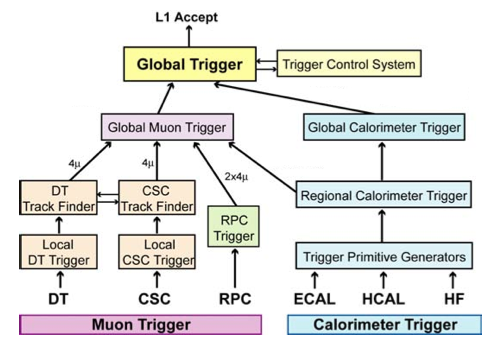
\includegraphics[width=0.8\textwidth]{\chthree/TriggerSystem.png}
 \end{center}
 \caption{\small  Architecture of the \Lone Trigger~\cite{Chatrchyan:2008zzk}.}
 \label{fig:TriggerSystem}
\end{figure}

%\section{The CMS detector simulation}
%
%For a detailed understanding on how interactions in proton-proton collisions at the LHC are observed by the CMS detector, a dedicated simulation of the whole detector and the subatomic interactions is needed [5]. Both the propagation of particles through the detector material as well as the response of the active detector components and their digital output need to be sim- ulated. The input to the detector simulation are collections of particles produced by MC event generators. The output is the digital signal from all detector components in the same format that is used for real data (RAW).
%The CMS simulation is based on the GEANT4 toolkit~\cite{Agostinelli:2002hh}. It allows modeling of the full detector geometry and the simulation of particles? propagation through magnetic fields as well as electromagnetic and hadronic interactions with the crossed material. The simulation is per- formed in two steps: the simulation step and the digitization step. In the simulation step, parti- cles are propagated through the detector allowing for interaction with detector material. Hits are produced on interaction with sensitive detector components. In the digitization step, the elec- tronic readout of these hits is simulated, taking into account resolution and detector response effects.
%
%The particles that are generated by the event generators are then propa-
%gated through the detector with the GEANT 4 [72,73] program, which simu-
%lates the detector response to these particles. Using a detailed model of the
%CMS detector including the geometries and materials, GEANT 4 generates
%the hits and particle showers that would happen in the subdetectors and sub-
%sequently simulates the response of the detector electronics to these signals.
%After the simulation by GEANT 4, the data format of a simulated event is
%the same as for the data, so that, from this point onward, the same software can
%be used for the reconstruction of data and simulation. Pileup is included in the
%samples by mixing randomly chosen minimum bias events with the simulated
%events to achieve the expected PU distribution, shown in Figure 2.4.

